\documentclass[10pt]{article}
\usepackage[T1]{fontenc}
\usepackage[utf8]{inputenc}
\usepackage[english]{babel}
\usepackage{lmodern}
\usepackage[a4paper,margin=20mm]{geometry}
\usepackage{graphicx,booktabs,array,amsmath,amssymb,xcolor}
\usepackage{microtype}
\usepackage[colorlinks=true,linkcolor=teal,urlcolor=teal,citecolor=teal]{hyperref}
\definecolor{Ink}{HTML}{172B43}
\definecolor{Best}{HTML}{157553}
\definecolor{Rust}{HTML}{AF4D35}
\newcommand{\best}[1]{\textcolor{Best}{\textbf{#1}}}
\newcommand{\worst}[1]{\textcolor{Rust}{#1}}
\graphicspath{{figures/}}
\newcommand{\PCOne}{12.60}
\newcommand{\PCTwo}{7.69}
\newcommand{\PCTogether}{20.29}
\newcommand{\PCSelected}{91.50}

\setlength{\parindent}{0pt}
\setlength{\parskip}{5pt}
\newcommand{\figcaption}[1]{{\footnotesize #1\par}}
\newcommand{\topic}[1]{\par\medskip\textbf{#1}\par}

\hypersetup{pdftitle={Task 2: supplementary figures}}
\begin{document}
\section*{Supplementary figures: parameter effects}
This appendix is separate from the one-page Task 2 report contribution. It is not automatically part of the five-page group report.
\begin{center}
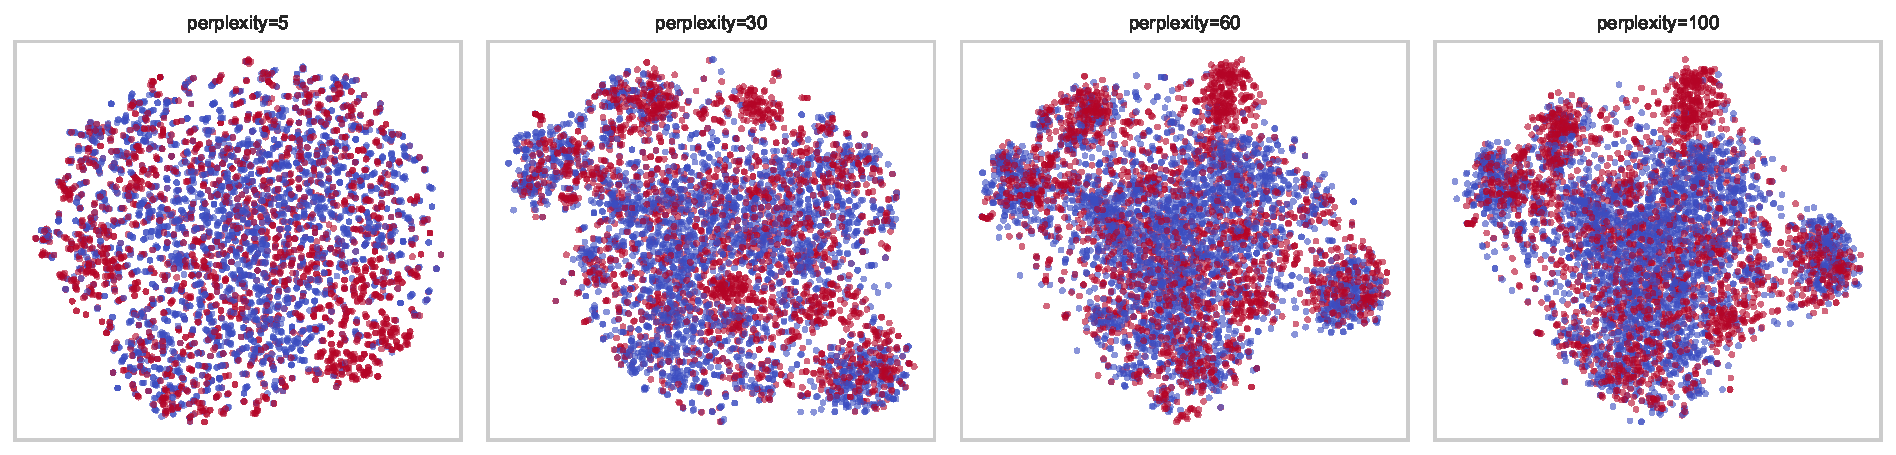
\includegraphics[width=.59\linewidth,height=73mm,keepaspectratio]{tsne_selected.pdf}
\end{center}
\figcaption{Figure A1. Selected original t-SNE sweep panels with enlarged parameter labels: perplexity 5, 30, 60 and 100. Same fixed 5,000 cells, 29 PCs and seed 42. Blue/cyan denote CMV-negative/positive donor labels. Trustworthiness at 60 is only slightly above the values at 50 and 100.}
\begin{center}
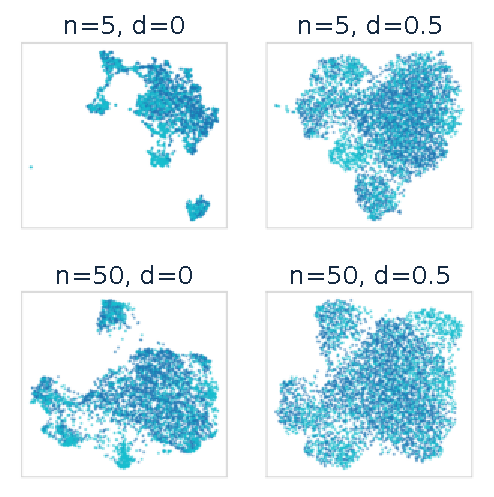
\includegraphics[width=.61\linewidth,height=83mm,keepaspectratio]{umap_selected.pdf}
\end{center}
\figcaption{Figure A2. Four settings from the original UMAP grid. Rows contrast 5 with 50 neighbours; columns contrast min\_dist=0 with 0.5. Smaller min\_dist permits tighter packing; n\_neighbors changes the graph's neighbourhood scale. Parameter-induced islands are not independently established cell types.}
\clearpage
\section*{Supplementary figures: marker expression}
\begin{center}
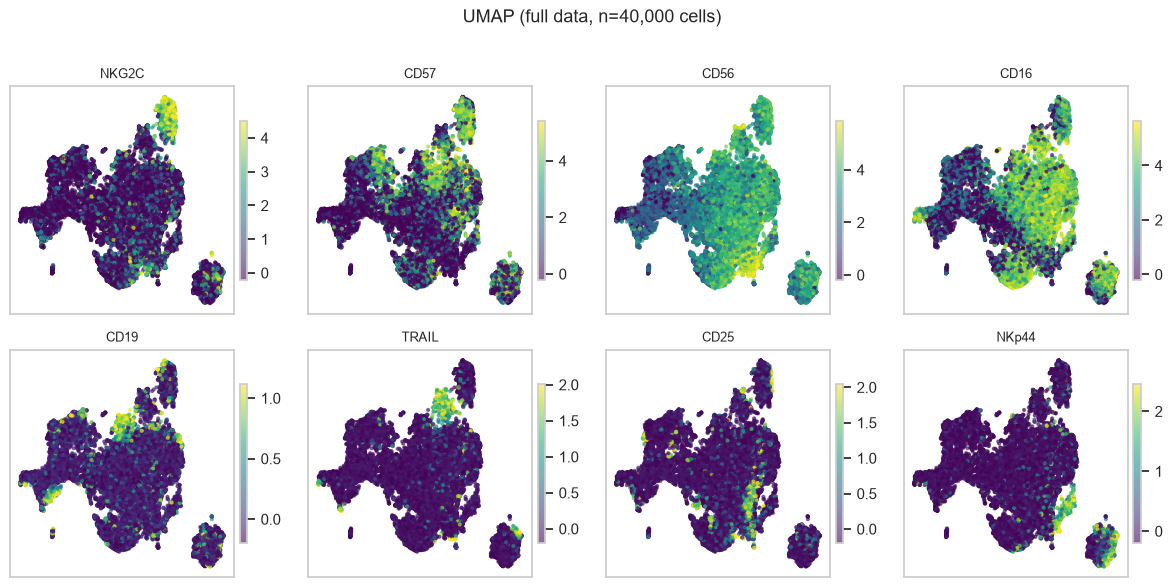
\includegraphics[width=\linewidth,height=91mm,keepaspectratio]{umap_markers.png}
\end{center}
\figcaption{Figure A3. Original UMAP marker overlays from notebook cell 41 (counting from 1), on the balanced 40,000-cell sample. Each panel colours the same points by a different arcsinh-transformed marker; colour limits are clipped at that marker's 1st/99th percentiles. Numerical scales therefore differ between markers.}
\begin{center}
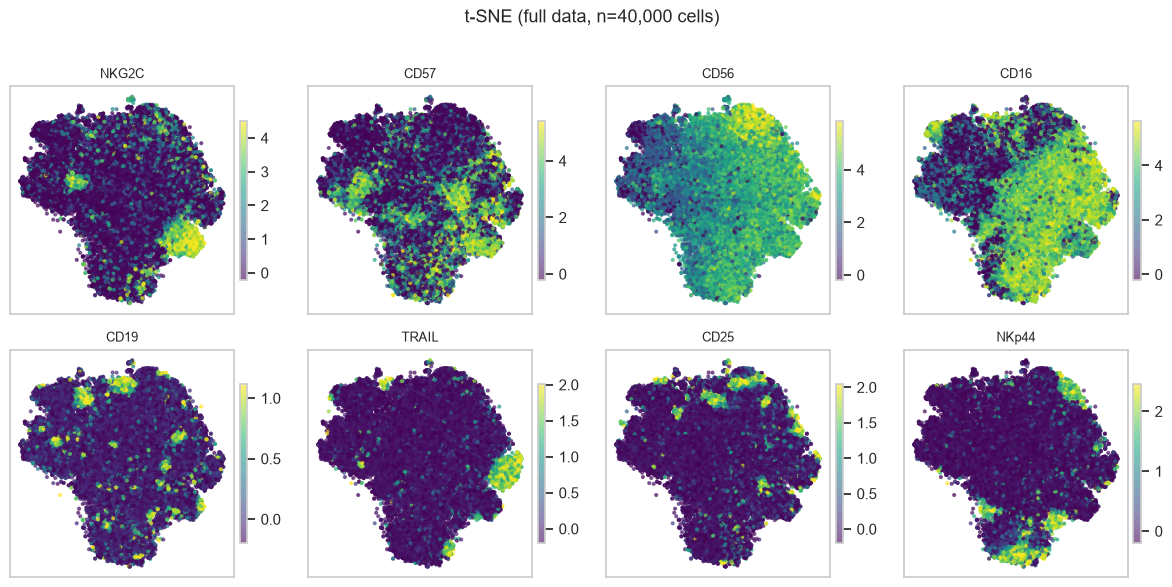
\includegraphics[width=\linewidth,height=91mm,keepaspectratio]{tsne_markers.png}
\end{center}
\figcaption{Figure A4. The same markers and cells on the saved t-SNE map. NKG2C/CD57 expression can guide follow-up of a memory-like NK phenotype, but expression gradients alone do not validate a functional adaptive population or label individual cells as CMV-infected. The plots' ``full data'' titles refer to the full balanced analysis sample, not all 261,593 available NK cells.}
\end{document}
